\section{Laplace Transformation}
\definition{Motivation}{Eine Transformation ermöglicht das Vereinfachen von 
Problemlösungen, indem das Problem in einem anderen 'Raum' gelöst wird.}

Beispiel:
\begin{equation*}
    \int \frac{x}{x^2+1} \text{d}x
\end{equation*}
Transformation: 
\begin{equation*}
    u = x^2 + 1 \Rightarrow \frac{\text{d}u}{\text{d}x}=2x\Rightarrow
    \text{d}x = \frac{\text{d}u}{2x}
\end{equation*}
Lösen:
\begin{equation*}
    \int \frac{1}{2u} \text{d}u = \frac{1}{2} \ln u
\end{equation*}
Rücktransformation:
\begin{equation*}
    \frac{1}{2} \ln \left( x^2+1 \right)
\end{equation*}

Der Laplace-Raum ist ein Raum, in dem Differentialgleichungen sehr einfach zu
lösen sind.

\subsection{Definition}
Annahme: Funktionen $f(t)$ sind so, dass
\begin{equation*}
    f(t)=0, \hspace{1em} t\leq0
\end{equation*}
\begin{center}
    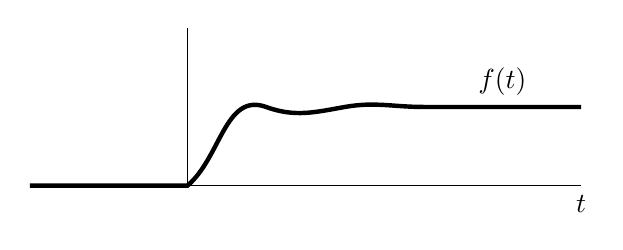
\begin{tikzpicture}
        \draw (0,2) -- (0,0) -- (5,0) node[below] {$t$};
        \draw[ultra thick] (-2,0) -- (0,0) 
            to[out=40,in=160] (1,1) 
            to[out=-20,in=190] (2,1)
            to[out=10,in=180] (3,1)
            -- (5,1) 
            node[pos=0.5,above] {$f(t)$};
    \end{tikzpicture}
\end{center}
\definition{Definition}{Laplace Transformation von $f(t)$}
\begin{equation*}
    \boxed{
        F(s) = \int_0^\infty f(t) e^{-st}\text{d}t
    }
\end{equation*}

Schreibweise:
\begin{eqnarr}
    F(s) &=&  \L (f(t)) \\
    F\tikzmark{a}(s) &\multimapdotbothB& f\tikzmark{b}(t)
\end{eqnarr}
\begin{center}
    \begin{tikzpicture}[overlay,remember picture]
        \node at (-2,0) (ta) {Bildfunktion};
        \node at (2,0) (tb) {Originalfunktion};
        \draw[->,thick] (ta) to (a);
        \draw[->,thick] (tb) to (b);
    \end{tikzpicture}
\end{center}

\bsp{Beispiele:}

\underline{Sprungfunktion}
\begin{equation*}
    \sigma (t) = \left\{ \begin{array}{c} 
            0 \text{ für } t<0\\
            1 \text{ für } t\geq0\\
    \end{array} \right.
\end{equation*}
\begin{center}
    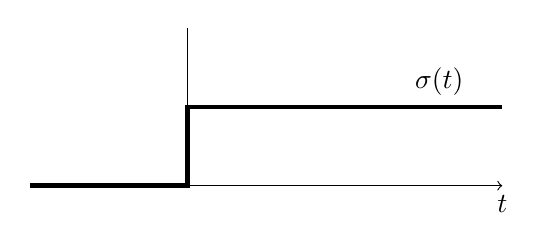
\begin{tikzpicture}
        \draw[->] (0,2) -- (0,0) -- (4,0) node[below] {$t$};
        \draw[ultra thick] (-2,0) -- (0,0) -- (0,1) -- (4,1)
            node[pos=0.8,above] {$\sigma(t)$};
    \end{tikzpicture}
\end{center}
\begin{eqnarr}
    \L \left( \sigma(t) \right) &=& \int_0^\infty e^{-st}dt \\
    &=&  \left. -\frac{1}{s} e^{-st}\right|_0^\infty \\
        &=& \frac{1}{s} \hspace{4em} \text{(falls Re} (s)>0)
\end{eqnarr}
\begin{equation*}
    \boxed{
        \frac{1}{s} \multimapdotbothB 1
    }
\end{equation*}
